\documentclass[titlepage]{article}

\usepackage[utf8]{inputenc}
\usepackage[T1]{fontenc}
\usepackage{listings}
\usepackage{color}
\usepackage{graphicx}
\usepackage[francais]{babel}
\definecolor{mygreen}{rgb}{0,0.6,0}
\definecolor{mygray}{rgb}{0.5,0.5,0.5}
\definecolor{mymauve}{rgb}{0.58,0,0.82}
\lstset{ 
  basicstyle=\footnotesize,        % the size of the fonts that are used for the code
  breakatwhitespace=false,         % sets if automatic breaks should only happen at whitespace
  breaklines=true,                 % sets automatic line breaking
  captionpos=b,                    % sets the caption-position to bottom
  commentstyle=\color{mygreen},    % comment style
  frame=single,	                   % adds a frame around the code
  keepspaces=true,                 % keeps spaces in text, useful for keeping indentation of code (possibly needs columns=flexible)
  keywordstyle=\color{blue},       % keyword style
  language=Bash,                 % the language of the code
  numbers=left,                    % where to put the line-numbers; possible values are (none, left, right)
  numbersep=5pt,                   % how far the line-numbers are from the code
  numberstyle=\tiny\color{mygray}, % the style that is used for the line-numbers
  rulecolor=\color{black},         % if not set, the frame-color may be changed on line-breaks within not-black text (e.g. comments (green here))
  showspaces=false,                % show spaces everywhere adding particular underscores; it overrides 'showstringspaces'
  showstringspaces=false,          % underline spaces within strings only
  showtabs=false,                  % show tabs within strings adding particular underscores
  stepnumber=1,                    % the step between two line-numbers. If it's 1, each line will be numbered
  stringstyle=\color{mymauve},     % string literal style
  tabsize=2,	                   % sets default tabsize to 2 spaces
  title=\lstname                   % show the filename of files included with \lstinputlisting; also try caption instead of title
}

\setlength{\parindent}{2em}
\setlength{\parskip}{.5em}

\begin{document}

	\title{Implémetation d'un serveur d'archives en Bash avec NetCat}
	\author{Antoine Prudhomme \\ \\ Mathilde Sandor}
	\date{\today}

	\maketitle

	\tableofcontents
	\newpage

	% ============ %
	% INTRODUCTION %
	% ============ %
	\section{Introduction}
	L'objectif du projet était d'implémenter un serveur d'archives sous Linux en Bash.
	Le serveur contient des archives, dans un format défini dans le sujet. 
	Un client peut intéragir avec le serveur au travers d'une commande shell, nommée \textbf{vsh}. :
	Cette commande possède 3 modes:
	\begin{itemize}  
	\item \textbf{list}, pour afficher l'ensemble des archives du serveur.
	\item \textbf{browse}, pour explorer une archive. Ce mode gère les commandes \textbf{pwd, cd, ls, rm et cat}.
	\item \textbf{extract}, qui permet d'extraire une archive depuis le serveur sur la machine cliente.
	\end{itemize}   

	% -------------- %
	% CLIENT SERVEUR %
	% -------------- % 
	\section{Modèle client serveur avec NetCat}
	
	\subsection{Netcat} 
	Pour implémenter le modèle client-serveur, nous avons utilisé l'utilitaire \textbf{NetCat} qui permet de gérer des sockets.
	Netcat permet d'écouter sur un port réseau, de parler sur un port réseau, mais aussi au serveur de répondre aux clients en utilisant un \textbf{named pipe}.

	% SERVEUR %
	\subsubsection{Implémentation d'un serveur avec Netcat}

	On utilise simplement cette commande
	\begin{lstlisting}
	nc -l -p $port
	\end{lstlisting}

	Le soucis, c'est qu'une fois la reqûete traitée par le serveur, netcat ferme la connexion, donc le serveur arrête d'écouter le port. Pour résoudre ce problème, on peut simplement mettre la commande ci-dessus dans une boucle infinie: tant que le serveur tourne, on relance l'écoute du port à chaque reqûete traitée.
	\begin{lstlisting}
	while true;
	do
		echo "server is listening on port $port"
		nc -lp $port
	done
	\end{lstlisting}

	Le serveur lit sur le socket, mais on souhaite également qu'il puisse écrire sur ce même socket. Pour cela, on crée un \textbf{named pipe}, que l'on nomme ici \textbf{backpipe}.
	\begin{lstlisting}
	if [ ! -e backpipe ];
	then
	    mkfifo backpipe
	fi

	while true;
	do
	    echo "server is listening on port $port"
	    nc -l $port < backpipe | echo "hello world" > backpipe
	done
	\end{lstlisting}

	Le script ci dessus renvoie \textit{"hello world"} à chaque requête d'un client.

	Mais le client ne se contentera pas de se connecter au serveur. Il va envoyer une commande \textbf{vsh} au serveur. Donc le serveur doit être capable dans un premier temps d'intercepter la reqûete, puis, après avoir fait ce qu'il avait à faire, écrire une réponse dans la socket à destination du client. Le code ci dessous permet de faire ça. 

	\begin{lstlisting}
	if [ ! -e backpipe ];
	then
	    mkfifo backpipe
	fi

	while true;
	do
	    echo "server is listening on port $port"
	    req=$(nc -lp $port)
	    nc -l $port < backpipe | echo "request: $req" > backpipe
	done
	\end{lstlisting}

	On a donc un code qui permet de créer un serveur capable de gérer des requêtes puis de retourner une réponse au client. Il reste donc à voir comment un client peut envoyer une requête au serveur.

	% client %
	\subsection{Implémentation d'un client avec Netcat}
	Le code d'un client est beaucoup plus simple que celui d'un serveur, puisque les seules actions qu'il a à faire sont:
	\begin{itemize}  
		\item se connecter au serveur 
		\item envoyer une requête
		\item se mettre en écoute pour attendre la réponse du serveur
	\end{itemize}

	Ci-dessous, le code du client (\textit{req.txt} est un fichier contenant la reqûete).

	\begin{lstlisting}
	nc $host $port < req.txt
	sleep 1s
	nc $host $port
	\end{lstlisting}

	\textit{Dans notre implémentation, nous utilisons le même port pour le client et pour le serveur}

	Nous avons donc un modèle client-serveur fonctionnel.

	% ----------------- %
	% STRUCTURE DU CODE %
	% ----------------- % 
	\subsection{Structure de notre code}

	Notre implémentation de VSH est basée sur le code client-serveur détaillé dans la section précédente.
	À la racine du projet, on trouve deux dossiers:
	\begin{itemize}  
		\item \textbf{client}, qui contient le code du client 
		\item \textbf{server}, qui contient le code du serveur
	\end{itemize}

	\textit{Les scripts du client sont totallement indépendants des scripts du serveurs.}

	% structure du serveur %
	\subsubsection{Structure du serveur}
	Le point d'entrée du serveur est le script \textbf{server.sh}. Le code de ce script est très similaire à celui présenté plus haut. La différence est qu'ici, on ne ne renvoie pas au client sa reqûete. La reqûete du client est parsée, et à l'aide d'un \textit{case}, on décide de ce qu'il faut faire.
	\begin{itemize}  
		\item Si la requête match un cas du \textit{case} différent du cas par défaut, on execute le \textit{sous script} du serveur qui correspond et on retourne au client ce que retourne ce sous script.
		\item Si la requête match le cas par défaut (donc que la reqûete n'est pas connue par le serveur) le serveur retourne un message pour indiquer que la commande est inconnue.
	\end{itemize}

	Pour lancer le serveur, il faut ouvrir un shell dans le repertoire \textbf{server} puis executer la commande suivante:

	\begin{lstlisting}
	bash server.sh $port
	\end{lstlisting}

	\textit{Les différents sous script sont détaillés dans les sections suivantes.}

	% structure du client %
	\subsubsection{Structure du client}

	Le point d'entré est le script \textbf{vsh} auquel on a retiré l'extension. Ainsi, en ajoutant son repertoire à la variable \textbf{PATH} on pourra utiliser \textbf{vsh} de la même manière que les commandes shell standard (\textbf{pwd, ls, ...}). \par
	\textit{Le fichier \textbf{README.md} explique comment ajouter \textbf{vsh} à \textbf{PATH}}

	Lorsque le script \textbf{vsh} est executé, on fait un choix en fonction de la valeur du premier paramètre donné par l'utilisateur.

	\begin{itemize}
		\item Si le 1er paramètre correspond à un mode vsh
		\begin{itemize}
			\item Si il y a tous les paramètres attendu, on execute le mode vsh
			\item Sinon, on affiche un message d'erreur
		\end{itemize}
		\item Sinon, on appel la fonction \textbf{usage} pour afficher l'aide
	\end{itemize}

	% ========= %
	% MODE HELP %
	% ========= %
	\section{help}

	Le mode \textbf{help} permet à l'utilisateur d'avoir des informations sur la commande \textbf{vsh}. 

	\begin{lstlisting}
	vsh --help
	\end{lstlisting}

	Ce qui est affiché à l'utilisateur une fois la commande ci dessus executée est le contenu de la fonction \textbf{usage}, qui décrit l'utilisation de la commande \textbf{vsh}. Cette fonction est définie dans le script \textbf{vsh} du repetoire \textbf{client}.

	\textit{Le mode \textbf{help} informe l'utilisateur sur comment executer le mode \textbf{browse}, mais ne donne pas d'informations sur les commandes du mode \textbf{browse}, car il possède sa propre fonction \textbf{help}, détaillée dans la section dédiée à \textbf{browse}}

	% ========== %
	% MODE LIST %
	% ========== %
	\section{list}

	\subsection{coté client}

	Si l'utilisateur a entré "client", on vérifie qu'il a fourni les 3 arguments. Si ce n'est pas le cas la commande vsh envoie un message d'erreur. Si tout est bien indiqué on envoie la demande au serveur.

	\subsection{coté serveur}

	On demande à lire tous les fichiers du dossier archive sans indiquer son chemin	

	\begin{lstlisting}
	find archives -type f -exec basename {} \;
	\end{lstlisting}

	% =========== %
	% MODE BROWSE %
	% =========== %
	\section{browse}

	Le mode \textbf{browse} permet à l'utilisateur de naviguer dans une archive du serveur.

	\begin{lstlisting}
	# $host: le serveur
	# $port: le port sur le serveur
	# $archive_name: le nom de l'archive dans laquelle on souhaite naviguer
	vsh -browse $host $port $archive_name
	\end{lstlisting}

	Ce mode fait entrer l'utilisateur dans un nouveau shell (Figure \ref{fig:browse}).

	\begin{figure}
  	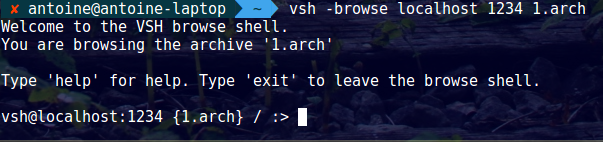
\includegraphics[width=\linewidth]{browse.png}
  	\caption{VSH Browse Shell}
  	\label{fig:browse}
	\end{figure}

	Dans un premier temps, un petit message est affiché à l'utilisateur, pour lui indiquer qu'il se trouve dans le shell VSH, et lui rappeler dans quelle archive il navigue. On lui dit également comment obtenir de l'aide et comment quitter le shell VSH.

	Le prompt donne différentes d'informations:
	\begin{itemize}  
		\item \textbf{vsh}: on se trouve dans le shell vsh
		\item \textbf{@localhost:1234}: le serveur et le port auquel on est connecté
		\item \textbf{{1.arch}}: l'archive dans laquelle on navigue
		\item notre emplacement actuel dans l'archive (ici, à la racine) 
	\end{itemize}

	Une fois dans ce shell, plusieurs commandes, présentées ci dessous, sont disponibles.

	\textit{Les chemins vers les fichiers ou répertoires peuvent être soit relatifs, soit absolus}

	\subsection{help}

	La commande \textbf{help} affiche l'aide, avec l'utilisation de chacune des commandes disponibles.

	\subsection{pwd}

	La commande \textbf{pwd} affiche le répertoire courant. Cette information est gardée côté client car c'est le client qui conserve l'état de sa connexion avec le serveur. Donc pour cette commande, aucune reqûete au serveur n'est requise, on affiche simplement le contenu de la variable qui contient le répertoire courant.

	\subsection{ls}

	La commande \textbf{ls} affiche le contenu d'un repertoire. Si aucun chemin n'est précisé, c'est le contenu du repertoire courant qui sera affiché.

	Côté serveur, on s'occupe de trouver les fichiers et répertoires contenu dans le repertoire demandé. Pour celà, l'algorithme va chercher la partie de l'archive qui définie le repertoire, c'est à dire de la ligne \textbf{directory} correspond au répertoire jusqu'au prochain symbole \textbf{@}. 

	Côté client, on parcours l'ensemble des lignes retournées par le serveur, qui décrivent le contenu du repertoire. Pour chacune de ces ligne, on regarde également si c'est un repertoire ou un fichier executable afin d'indiquer cette information à l'affichage.

	\subsection{cat}

	La commande \textbf{cat} affiche le contenu d'un fichier. Si aucune fichier n'est donné en paramètre, alors on affiche un message d'erreur.

	Côté serveur, on commence par trouver la ligne de l'archive décrivant le fichier dans l'archive. Pour celà, il nous faut deux informations:
	\begin{itemize}  
		\item Le nom du fichier   
		\item Le répertoire dans lequel il se trouve. Car deux repertoires différents peuvent tout à fait contenir un fichier portant le même nom.   
	\end{itemize}

	Dans un premier temps, on récupère le contenu du répertoire qui contient le fichier cherché. Pour celà, on utilise la commande \textbf{ls}. Puis on parcours les lignes retournées à la recherche du fichier désiré.

	\begin{itemize}
		\item Si le fichier n'a pas été trouvé, alors on retourne un code d'erreur.
		\item Sinon si le fichier possède un contenu (sa description contient des informations supplémentaires), alors on affiche les lignes de l'archive correspondantes au contenu de ce fichier.
	\end{itemize}

	Côté client, on a juste à vérifier le contenu de la réponse du serveur. Si la réponse contient le code d'erreur, alors on affiche un message à l'utilisateur l'informant que le fichier n'existe pas. Dans le cas contraire, on affiche la réponse du serveur qui est le contenu du fichier demandé.

	\subsection{rm}

	La commande \textbf{rm} supprime le fichier donné. Si aucun fichier n'est donné, un message d'erreur est affiché à l'utilisateur.

	Tout le travail se fait côté serveur. Pour supprimer un fichier de l'archive, on retrouver les mêmes problématiques que \textbf{cat}, donc on commence de la même manière, en utilisant \textbf{ls} et en regardant les informations complétementaires. Mais cette fois, au lieu d'afficher les lignes de l'archive correspondantes au contenu du fichier, on va les remplacer par des lignes vides. Puis on fait de même pour la ligne qui décrit le fichier dans le header de l'archive. Et voilà, le fichier a été éffacé de l'archive.

	Cette solution n'est pas optimale au sens où les lignes vides sont inutiles, et chacune de ces lignes augmente la taille de l'archive de 1 octet. Mais l'avantage de cette technique est que l'algorithme pour supprimer un fichier est très simple, car il n'y a pas besoin de reindexer les lignes dans l'archive et les informations complémentaires de chaque fichier.

	\subsection{rmdir}

	La commande \textbf{rmdir} supprime le répertoire donné. Si aucun repertoire n'est donné, un message d'erreur est affiché à l'utilisateur.

	De même que pour \textbf{rm}, tout le travail se fait côté serveur.

	Un répertoire pouvant contenir des fichiers et d'autres répertoires, on utilise la commande \textbf{rm} dans \textbf{rmdir} afin de ne pas réécrire de code pour la suppression de fichiers dans l'archive.

	Lorsque l'on supprime un répertoire, il faut penser que les répertoires qu'il contient (ses enfants directs) peuvent aussi contenir des répertoires. 

	Pour chaque déclaration de répertoire dans le header (\textbf{directory ...}) qui est un enfant du répertoire à supprimer ou le repertoire à supprimer lui même, on supprime tous les contenu des fichiers de ce répertoire puis on remplace toutes les lignes de la définition de se repertoire par des lignes vides.

	De même que pour la suppression de fichier, l'algorithme n'est pas optimal mais il est très simple.  

	% ============ %
	% MODE EXTRACT %
	% ============ %
	\section{extract}

	Le mode extract permet à l’utilisateur d’extraire une archive. Ici le serveur ne sert qu’à transmettre l’addresse de l’archive si elle existe. Et un code d’erreur si ce n’est pas le cas. 

	Le reste du travail se fait coté client. Si le serveur envoie un code d’erreur, le client envoie un message d’erreur. Sinon, le client va extraire l’archive comme ci-suit.

	\subsection{Outils utilisés}

	Nous récupérons le début du header et le début du corps des fichiers grâce aux premieres indications de l’archives. Nous récupérons aussi la taille totale de l’archive afin de ne pas faire de boucle infinie.

	\begin{lstlisting}
		header_start=$(echo $first_line | cut -d ":" -f 1)
		body_start=$(echo $first_line | cut -d ":" -f 2) 
		extracted_length=$(wc -l $VSH_CLIENT_RES | cut -d " " -f 1)
	\end{lstlisting}

	Par la suite, nous aurons aussi besoin d’une fonction capable de transformer les permissions données sous forme entière (-rwxrwxrwx) en forme numérique (777). La fonction lit chaque caractère de la ligne de permission et offre des points à ceux qui ne sont pas « - ». Les variables user, group, et owner cumulent chacune les points qui les concernent et obtiennent une valeur définitive.

	\begin{lstlisting}
	p=$1
	user=0
	group=0
	owner=0
	[[ ${p:1:1} != "-" ]] && user=$(($user+4))
	[[ ${p:2:1} != "-" ]] && user=$(($user+2))
	[[ ${p:3:1} != "-" ]] && user=$(($user+1))
	\end{lstlisting}

	\subsection{Extraction des fichiers et dossiers}

	On utilise un read line pour parcourir le header et un grep pour connaitre la nature de l’élément de la ligne :
	\begin{itemize}
%		\item Si on lit un dossier (directory), ce dossier devient notre dossier courant (current_dir), et on le crée s’il n’existe pas déjà.
%		\item Si on lit un sous-dossier, on l’associe à la variable sub_dir, et on le crée en respectant son adresse. 
%		\item \begin{lstlisting}
%		sub_dir_path="$current_dir/$sub_dir"
%		mkdir -p $sub_dir_path	
%				\end{lstlisting}
%		\item On lui attribue les permissions qui lui reviennent grace à la fonction décrite plus haut en passant en argument les droits du fichier.
%		\item Si on lit un fichier, on sépare les informations de la ligne en parties  (définies par les espaces):
%%			\item Le nom, qui nous permet de crée le fichier.
%			\item \begin{lstlisting}
%			file_path="$current_dir/${parts[0]}"
%			touch $file_path
%					\end{lstlisting}			
%			\item Les permissions, que nous traduisons grâce à notre fonction, puis que nous attribuons au fichier.
%			\item S’il y a 5 parties, c’est que le fichier contient du texte. Dans ce cas on lit les 2 dernières parties. Elles décrivent où se situent le texte et les lignes qu’il contient.
%			\end{itemize}
	\end{itemize}


\end{document}